\documentclass[aspectratio=169,10pt]{beamer}
\usetheme{metropolis}
\usepackage{appendixnumberbeamer}
\usepackage{booktabs}
\usepackage{amsmath,amssymb}
\usepackage{tikz}
\usetikzlibrary{arrows.meta,positioning,calc,decorations.pathreplacing,shapes.geometric,fit}
\usepackage{pgfplots}
\pgfplotsset{compat=1.18}
\usepackage{xcolor}
\usepackage{multicol}
\usepackage{graphicx}
\usepackage{hyperref}
\hypersetup{colorlinks=true,urlcolor=columbia,linkcolor=columbia}

\definecolor{columbia}{RGB}{29,79,145}
\definecolor{columbialight}{RGB}{117,170,219}
\definecolor{columbiaaccent}{RGB}{210,73,42}
\definecolor{columbiagray}{RGB}{117,117,117}
\definecolor{softbg}{RGB}{245,245,250}
\definecolor{hlgreen}{RGB}{46,139,87}

\setbeamercolor{frametitle}{bg=columbia,fg=white}
\setbeamercolor{progress bar}{fg=columbiaaccent}
\setbeamercolor{alerted text}{fg=columbiaaccent}
\setbeamercolor{block title}{bg=columbia,fg=white}
\setbeamercolor{block body}{bg=softbg}
\setbeamerfont{title}{size=\Large,series=\bfseries}
\setbeamerfont{subtitle}{size=\normalsize}
\graphicspath{{./figures/}}

\title{Lecture 27: Modern Biological AI}
\subtitle{BINF 4002 --- Machine Learning for Health}
\author{Matthew McDermott}
\institute{Dept.\ of Biomedical Informatics, Columbia University}
\date{April 28, 2026}

\begin{document}
\begin{frame}[noframenumbering]\maketitle\end{frame}

\begin{frame}{Where We Are}
\textbf{Three lectures on biological and molecular data:}
\begin{itemize}
    \item[\textcolor{columbiagray}{$\bullet$}] L25: DNA, genetics, gene regulation + classical analysis (GWAS, PRS, eQTL)
    \item[\textcolor{columbiagray}{$\bullet$}] L26: Proteins, molecules, structural biology + classical methods (MSA, SIFT, fingerprints, docking)
    \item[\textcolor{columbiaaccent}{$\to$}] \alert{L27: Modern Biological AI} $\gets$ \textbf{today}
\end{itemize}
\vspace{0.3em}
\textbf{L25--26:} biology interleaved with classical methods at each level.\\
\textbf{Today:} what deep learning adds---unified across all biological levels.
\end{frame}

\begin{frame}{Today's Outline}
\begin{enumerate}
    \item \textbf{Protein Language Models}---masked LM on amino acid sequences; zero-shot variant effect prediction
    \item \textbf{From Sequences to Structures}---MSA Transformer, AlphaFold, and the progression from single-sequence to alignment-based to structure-predicting models
    \item \textbf{Genomic Sequence Models}---predicting gene expression from DNA; the evaluation gap between reference prediction and variant effects
    \item \textbf{3D Molecular Models}---why 2D graphs (Lab 12) aren't enough; chirality and geometry-aware architectures
    \item \textbf{Designing New Biology}---the inverse problem: generating proteins with desired structure and function
\end{enumerate}
\end{frame}

\section{Protein Language Models}

\begin{frame}{ESM-2: Masked Language Modeling on Proteins}
\textbf{ESM} (Evolutionary Scale Modeling) is a family of protein language models from Meta AI. Train a transformer on protein sequences using BERT's masked prediction objective---but on the 20-letter amino acid alphabet.

\vspace{0.2em}
\textbf{Training:} Mask 15\% of amino acids, predict from context. Trained on UniRef50/D ($\sim$65M sequence clusters). No structural or functional labels.

\vspace{0.2em}
\textbf{What it learns} (without explicit supervision):
\begin{itemize}
    \item Evolutionary constraint (conserved residues harder to mask)
    \item Coevolutionary patterns (co-varying positions $\to$ 3D contacts)
    \item Functional motifs (active sites, binding regions)
\end{itemize}

\vspace{0.1em}
{\small Lin et al., 2023. Same paradigm as BERT $\to$ ClinicalBERT $\to$ ESM-2, but on the protein alphabet.}
\end{frame}

\begin{frame}{ESM-2: Key Results}
\centering
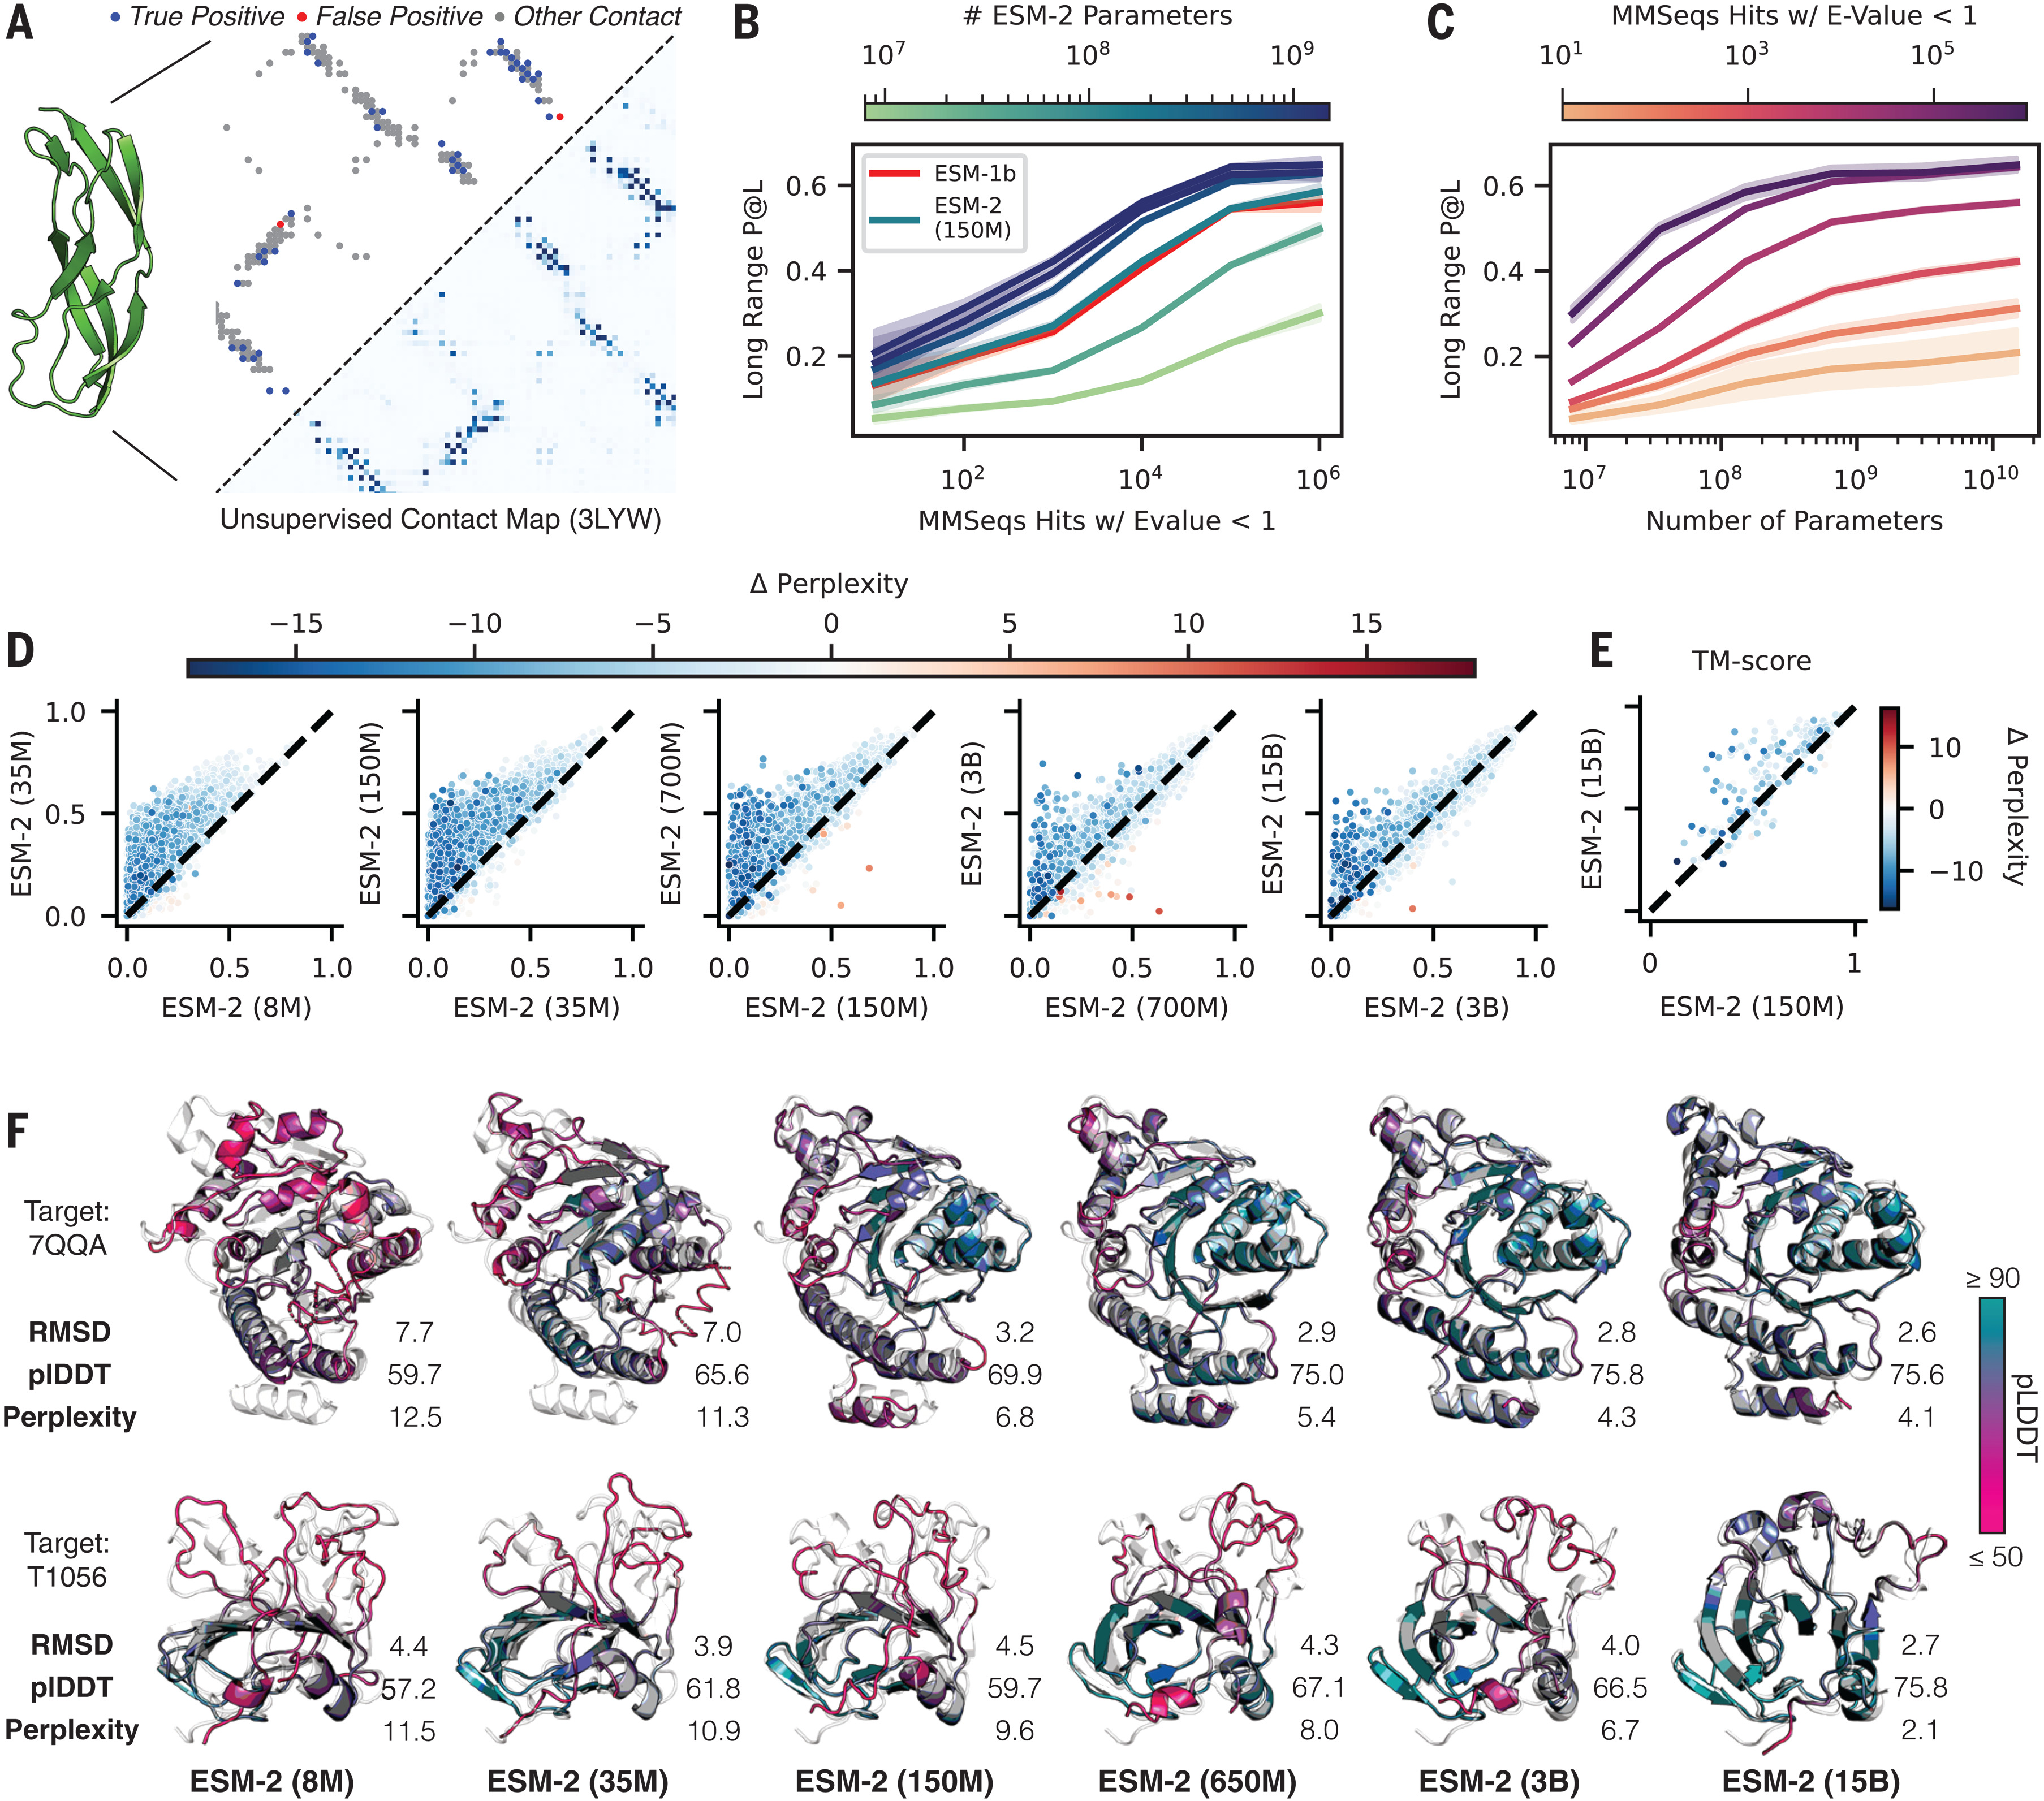
\includegraphics[width=\textwidth,height=0.90\textheight,keepaspectratio]{esm_fig}

\end{frame}

\begin{frame}{ESM Attention Recovers 3D Contacts}
\textbf{Rao et al.\ (2021):} Showed that transformer protein LM attention heads can learn residue--residue contacts from unsupervised LM objectives---\emph{without structural supervision}.

\begin{itemize}
    \item Published analyses used selective head combinations and learned contact predictors
    \item Published result (ESM-1b/650M): $\sim$50\% top-$L$/5 precision on long-range contacts
    \item DCA extracts the same signal from the MSA explicitly; ESM learns it implicitly
\end{itemize}

\vspace{0.2em}
The notebook includes a simplified classroom demonstration (average all heads, APC-correct) on ubiquitin. The signal is weak at classroom scale (35M model)---see the published figure on the next slide for what larger models achieve.
\end{frame}

\begin{frame}{Protein Language Models Naturally Predict 3DStructure}
\centering
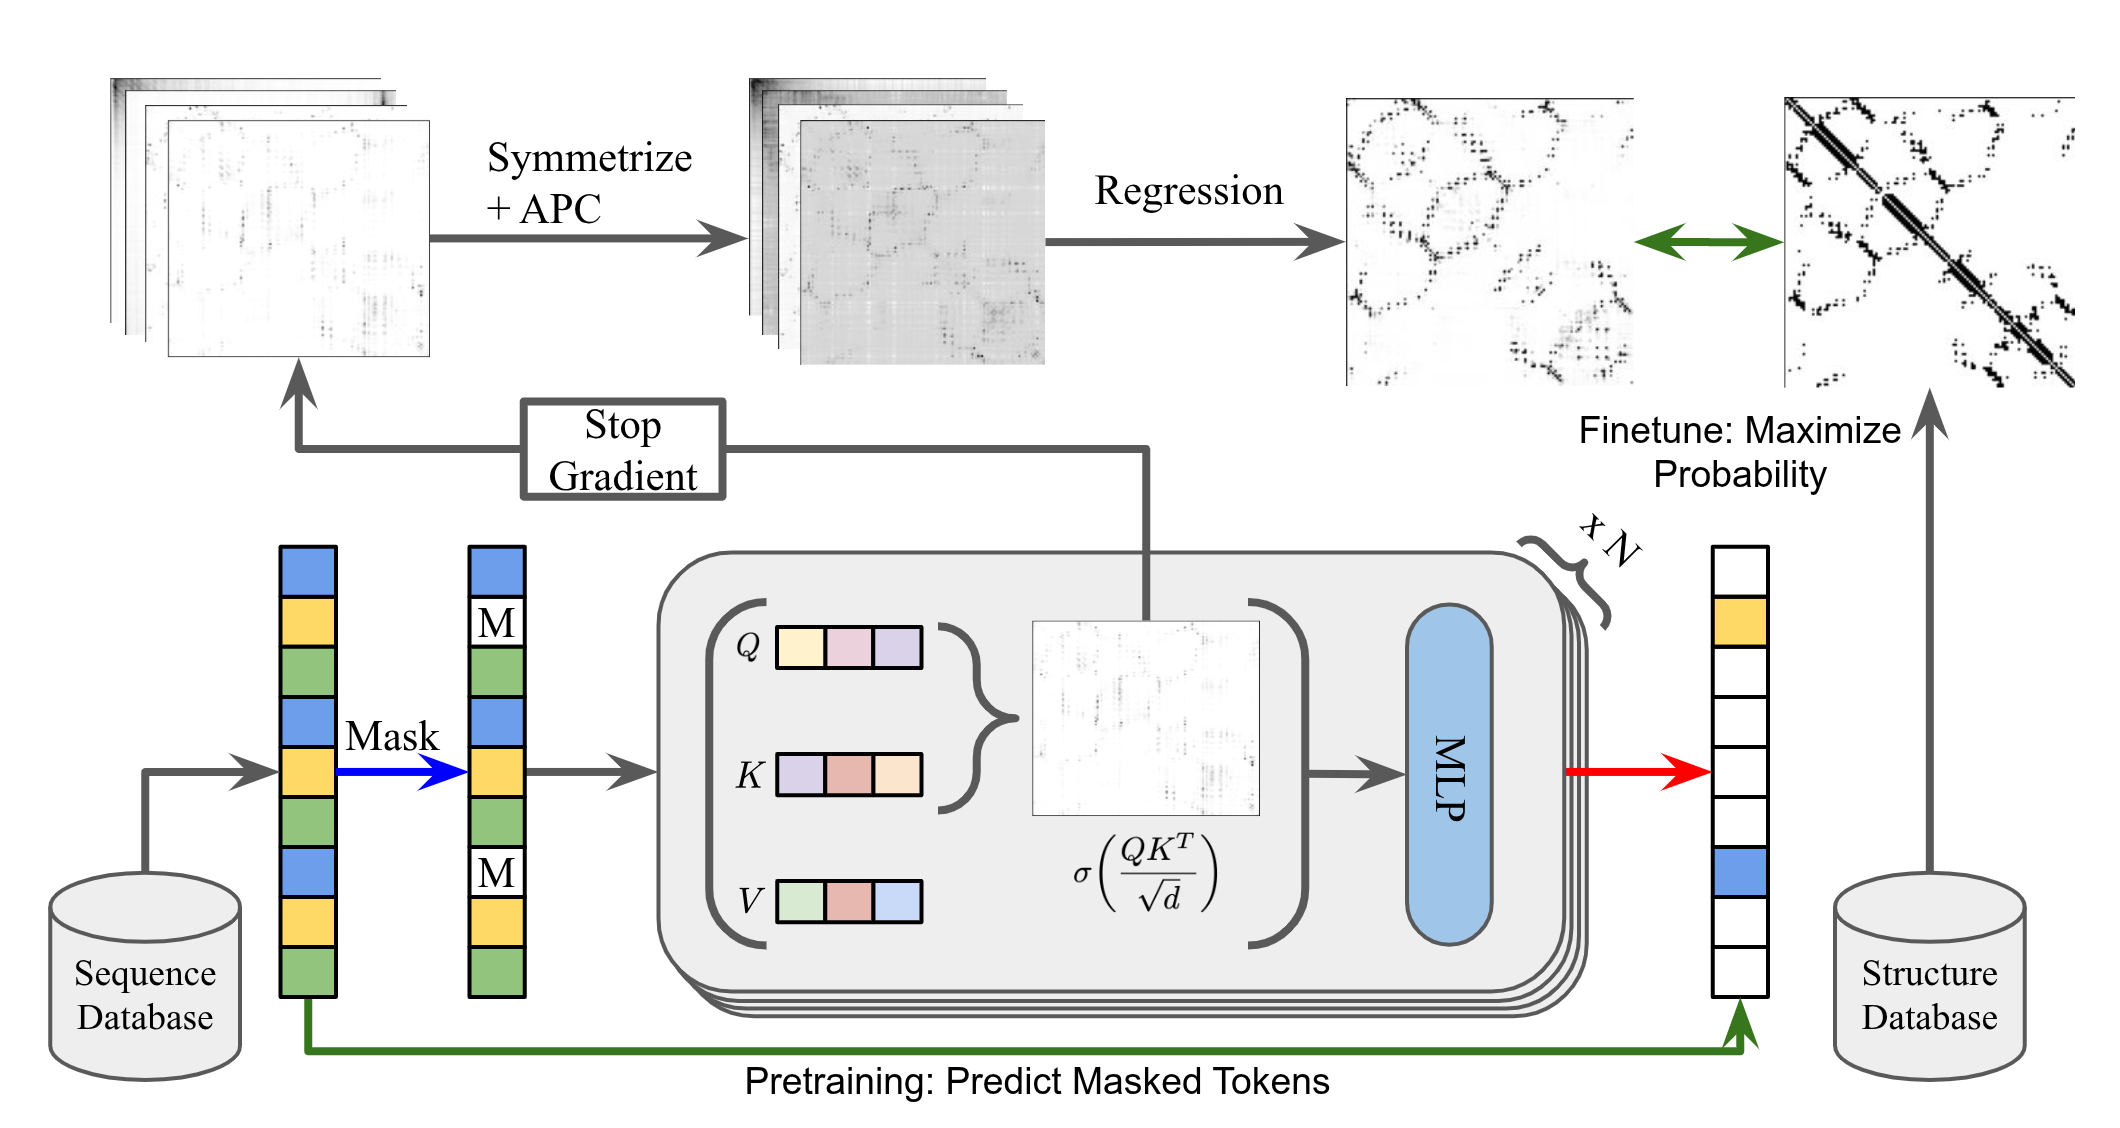
\includegraphics[width=\textwidth,height=0.70\textheight,keepaspectratio]{esm_contacts}

\end{frame}

\begin{frame}{Variant Effect Prediction: Zero-Shot}
\textbf{Idea:} Score a mutation by how much it reduces ESM's predicted probability:
$$\Delta\text{score} = \log P(\text{mut} \mid \text{context}) - \log P(\text{wt} \mid \text{context})$$
\begin{itemize}
    \item Low score $\to$ mutation violates evolutionary constraint $\to$ likely damaging
    \item SIFT uses MSA conservation; PolyPhen adds structure features. ESM zero-shot scoring captures sequence plausibility under a language model---related but not equivalent to these classical approaches.
    \item \textbf{Caveat:} Evolutionary plausibility $\neq$ pathogenicity. Gain-of-function mutations can look ``allowed.'' Context dependence is invisible.
\end{itemize}
\vspace{0.1em}
{\small Notebook Fig.~2: ClinVar-sourced HBB mutations (including sickle cell E6V). The 35M model shows partial separation; ESM-650M performs better on benchmarks like ProteinGym.}
\end{frame}

% \begin{frame}{Variant Effect Scoring (Notebook Fig.~2)}
% \centering
% 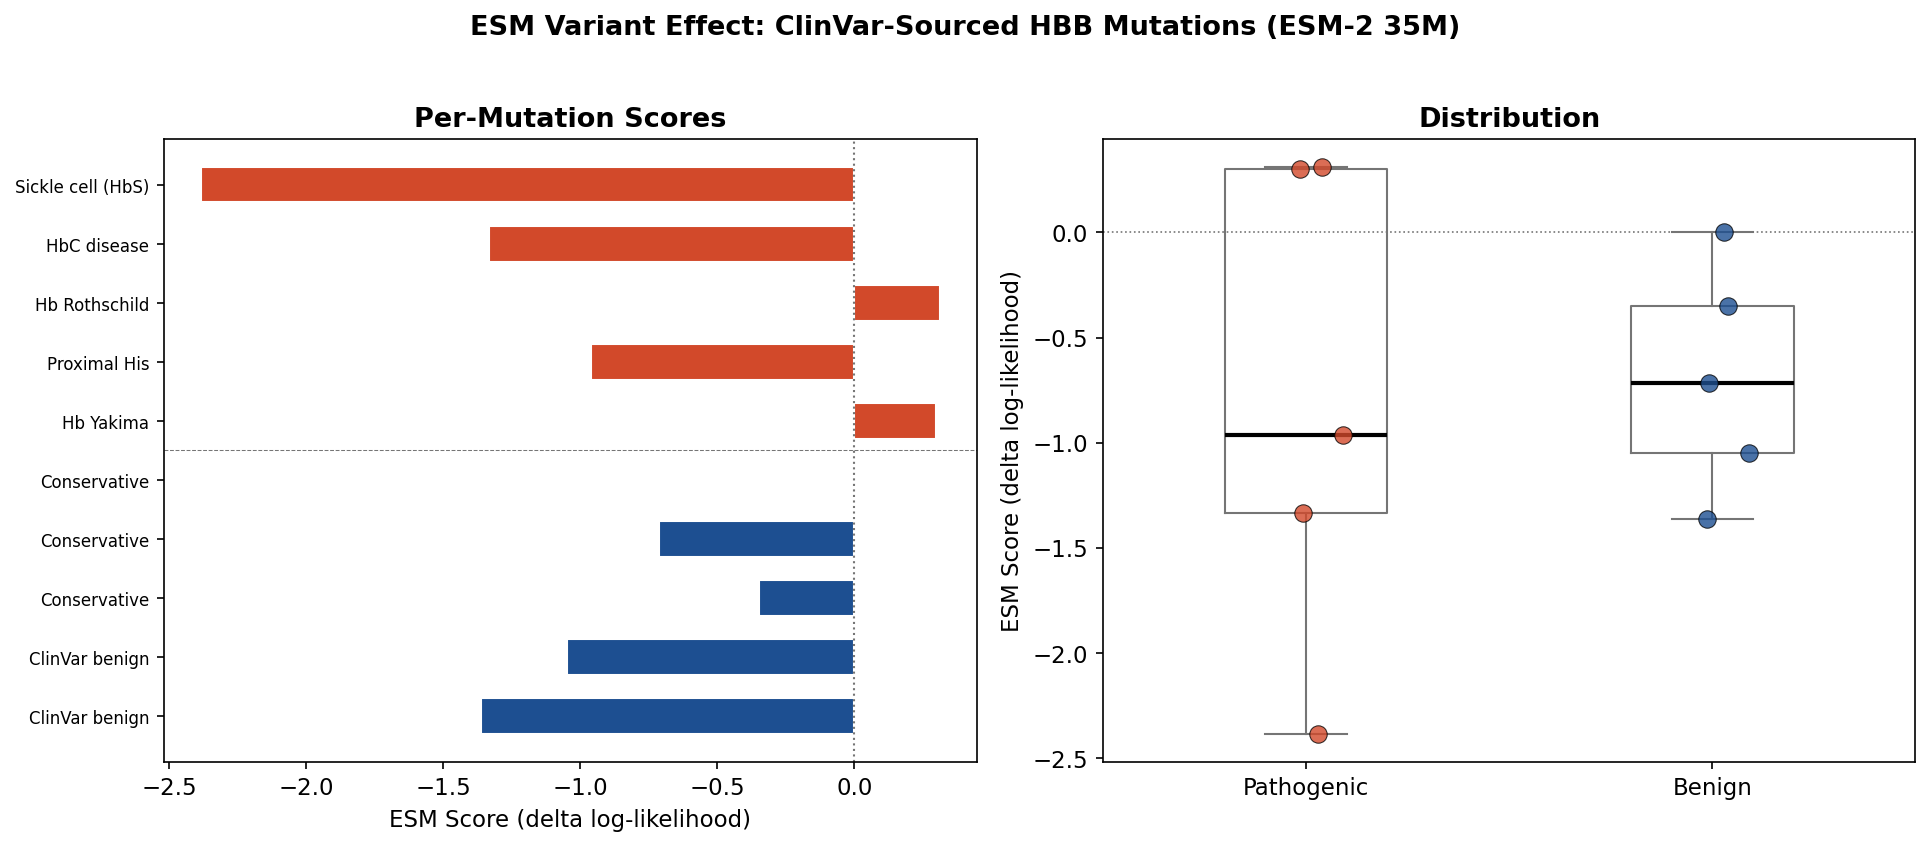
\includegraphics[width=\textwidth,height=0.65\textheight,keepaspectratio]{fig2_variant_effect.png}

% \vspace{-0.3em}
% {\scriptsize ClinVar-sourced HBB mutations scored by ESM-2 (35M). Some canonical pathogenic mutations (E6V, E6K) receive strongly negative scores, but separation is poor in this small classroom example---some pathogenic mutations score near zero. This is the point: sequence plausibility is not clinical pathogenicity.}
% \end{frame}

\begin{frame}{What Protein LMs Get Wrong}
\begin{enumerate}[<+->]
    \item \textbf{Plausibility $\neq$ pathogenicity:} Gain-of-function mutations look ``allowed'' but cause disease.
    \item \textbf{Conservation $\neq$ function:} Highly conserved sites may be structural, not functional.
    \item \textbf{Underrepresented families:} Viral, orphan, and synthetic proteins have poor coverage.
    \item \textbf{Context dependence:} Same protein, different tissue $\to$ different impact. Invisible to the model.
    \item \textbf{MSA-based methods often outperform:} Explicit MSA methods sometimes beat single-sequence ESM. What ESM learns beyond MSA statistics remains an open question.
\end{enumerate}
\end{frame}

\section{From Sequences to Structures}

\begin{frame}{ESM's Core Limitation}
ESM treats each protein sequence \textbf{independently}---one sequence in, one embedding out.

\vspace{0.3em}
But proteins didn't evolve independently. They share common ancestors, and \textbf{the pattern of covariation across related sequences} encodes structural and functional information that no single sequence contains.

\vspace{0.3em}
\textbf{The mismatch:} Evolution is a \emph{branching} process (phylogenetic tree), but ESM models it as a \emph{sequential} process (left-to-right masked prediction on individual sequences). ESM captures the \emph{marginal distribution} of amino acids at each position, but not the \emph{joint distribution} across homologous sequences.

% \vspace{0.3em}
% \textbf{Recall L26:} DCA (Direct Coupling Analysis) extracts coevolutionary signal from the MSA directly. Can we build a transformer that does the same---but learns from the data?
\end{frame}

\begin{frame}{MSA Transformer: Attention Over Alignments}
\begin{center}
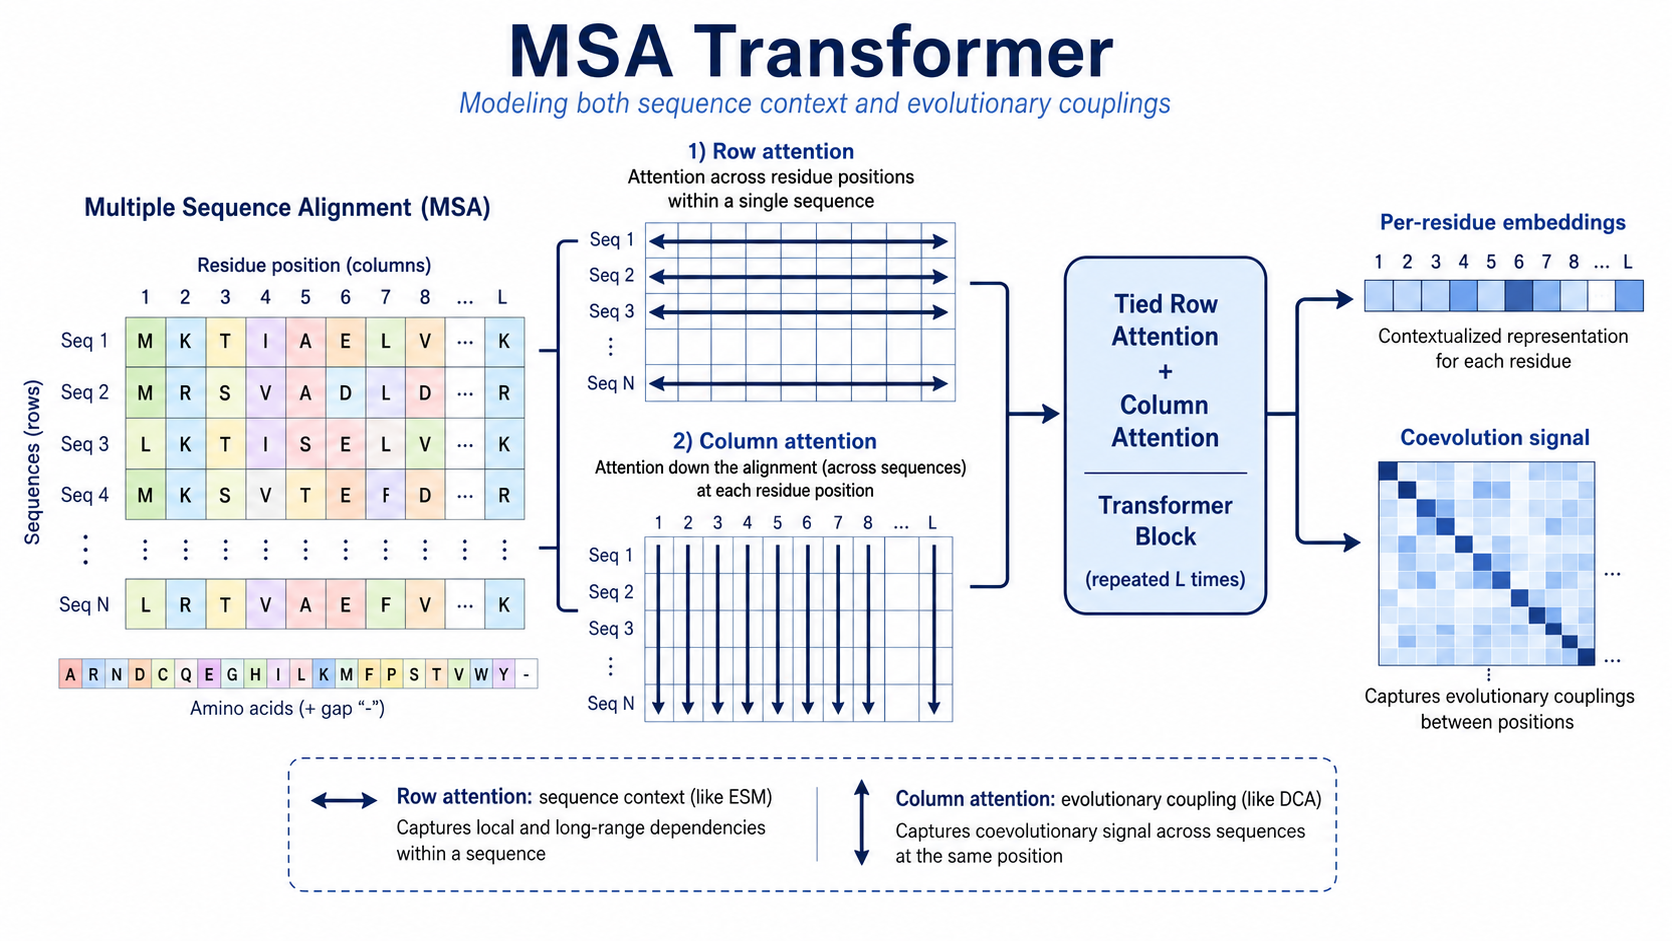
\includegraphics[width=\textwidth,height=0.58\textheight,keepaspectratio]{msa_transformer.png}
\end{center}

\vspace{-0.5em}
{\scriptsize Rao et al.\ (2021). Instead of processing one sequence at a time, the MSA Transformer processes the \emph{entire alignment} as a 2D input. \textbf{Row attention} (horizontal) captures sequence context within each protein---like ESM. \textbf{Column attention} (vertical) captures coevolutionary coupling across species at each position---like DCA. The model learns both simultaneously.}
\end{frame}

\begin{frame}{Why This Matters: From MSA Transformer to AlphaFold}
\textbf{MSA Transformer} showed that processing alignments with axial attention recovers contacts better than either single-sequence LMs (ESM) or classical coevolution (DCA) alone.

\vspace{0.3em}
\textbf{AlphaFold 2's Evoformer} takes this idea much further:
\begin{itemize}
    \item Same axial attention over MSA rows and columns
    \item Adds a \textbf{pair representation}---an explicit residue $\times$ residue matrix that tracks pairwise relationships
    \item Adds \textbf{structural supervision}---trained end-to-end to predict 3D coordinates, not just contacts
    \item Adds \textbf{template information}---known homologous structures, when available
\end{itemize}

\vspace{0.2em}
{\small The progression: ESM (single sequence) $\to$ MSA Transformer (alignment, axial attention) $\to$ Evoformer (alignment + pair repr.\ + structural supervision). Each step incorporates more of the evolutionary and structural signal.}
\end{frame}

\begin{frame}{AlphaFold 2 (DeepMind, Jumper et al.\ 2021): Nobel Prize in Chemistry 2024.}

\begin{center}
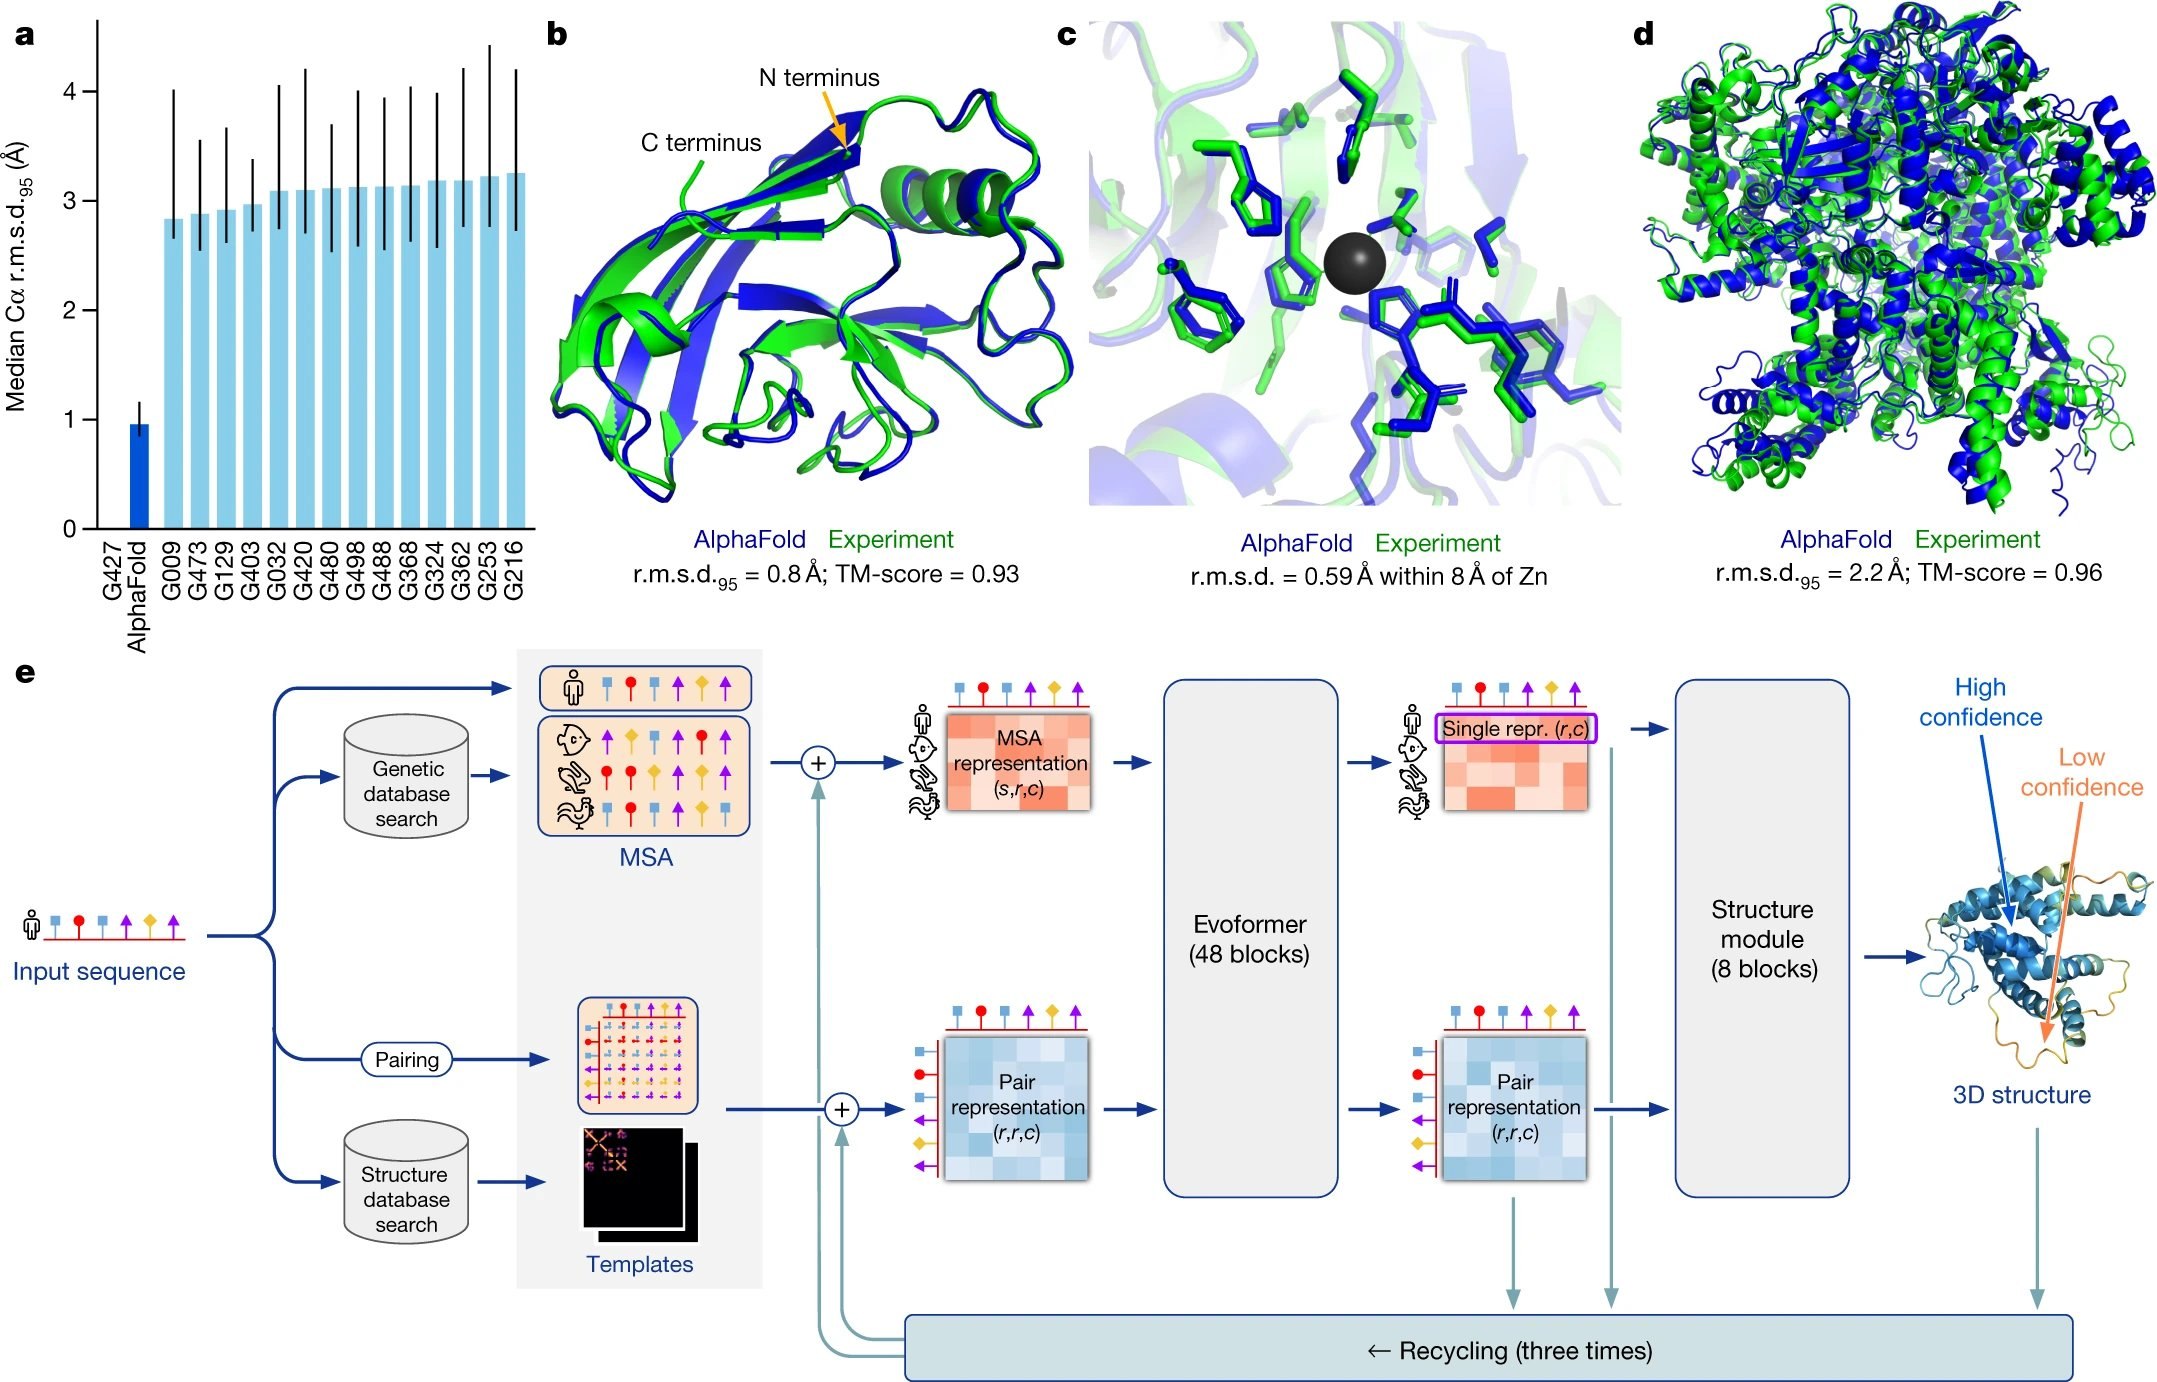
\includegraphics[width=\textwidth,height=0.7\textheight,keepaspectratio]{alphafold_fig1.png}
\end{center}

\vspace{-0.5em}
{\scriptsize Jumper et al., \textit{Nature} 596, 583--589 (2021). (a) CASP14 accuracy. (b--d) Predicted vs.\ experimental structures. (e) Full architecture: MSA + templates $\to$ Evoformer $\to$ structure module $\to$ 3D coordinates, with $3\times$ recycling.}% Paper: \texttt{doi.org/10.1038/s41586-021-03819-2}}
\end{frame}

\begin{frame}{What AlphaFold Gets Right---and Wrong}
\begin{columns}[T]
\column{0.48\textwidth}
\textbf{Right:}
\begin{itemize}
    \item Median GDT $\sim$92 on CASP14
    \item Globular, single-domain proteins
    \item 200M+ structures in AFDB
    \item Predict first, validate experimentally
\end{itemize}
\column{0.48\textwidth}
\textbf{Not designed / reliable for:}
\begin{itemize}
    \item Conformational ensembles (proteins move)
    \item Intrinsically disordered regions (low pLDDT is often \emph{correct}: no stable structure exists)
    \item Protein--protein interfaces
    \item Small-molecule binding geometry
    \item Mutation effects on dynamics
\end{itemize}
\end{columns}
\vspace{0.2em}
\textbf{Confidence scores are essential:} pLDDT (per-residue local confidence) and PAE (predicted aligned error, useful for domain orientation and complexes). Low-confidence regions are not just errors---they often mark genuine biological flexibility.
\end{frame}

\begin{frame}{AlphaFold Confidence: pLDDT (Notebook Fig.~3)}
\centering
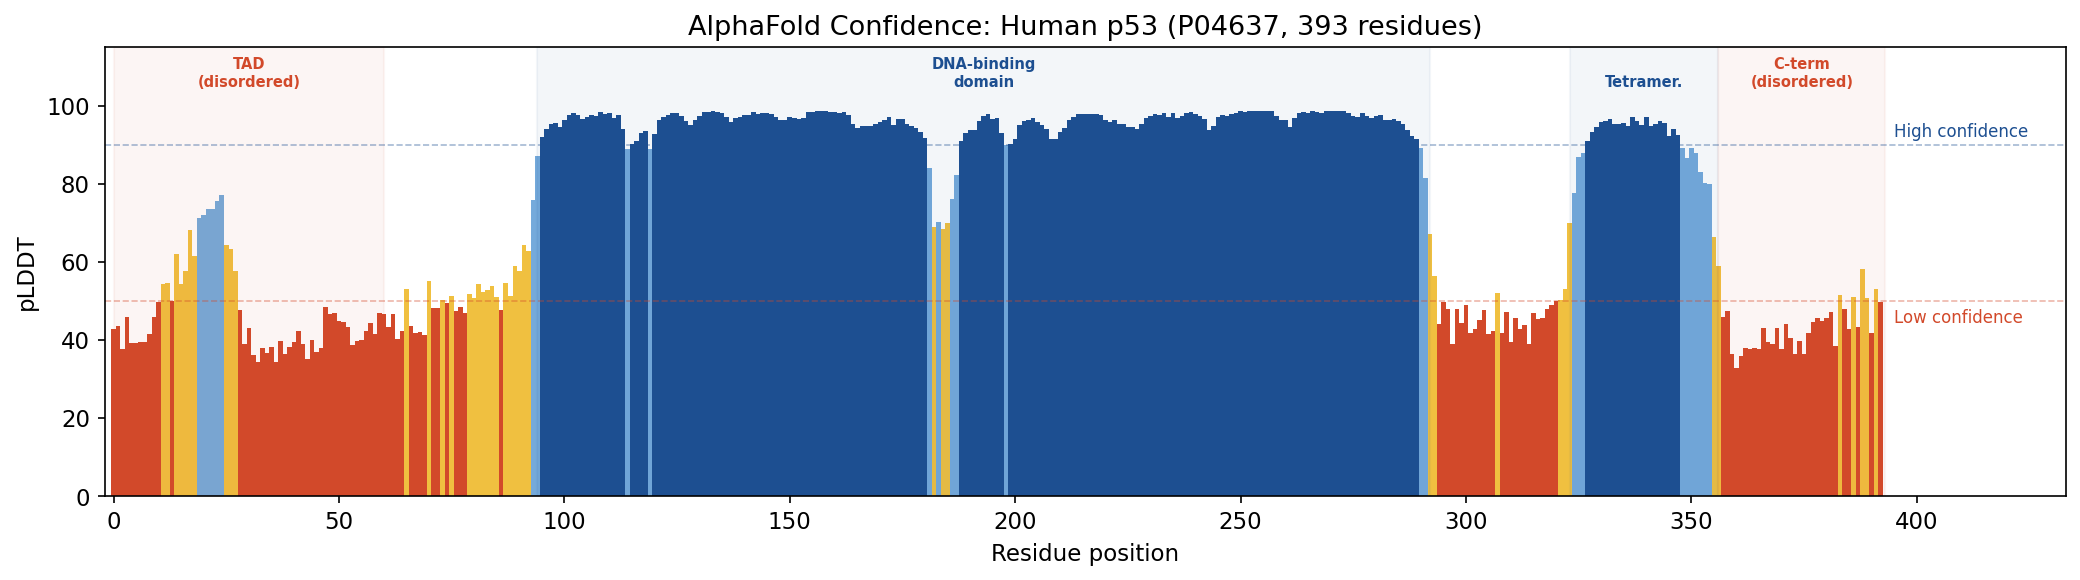
\includegraphics[width=\textwidth,height=0.65\textheight,keepaspectratio]{fig3_alphafold_plddt.png}

\vspace{-0.3em}
{\scriptsize Per-residue pLDDT for human p53 (AFDB). Blue: high confidence ($>$90). Red: low ($<$50, likely disordered). The confidence map---not just the structure---is the deliverable.}
\end{frame}

\begin{frame}{The AlphaFold Database and Beyond}
\textbf{AFDB:} 200M+ predicted structures. But pLDDT $\neq$ accuracy, and most can't be validated.
\vspace{0.2em}
\begin{center}
\renewcommand{\arraystretch}{1.15}
{\small
\begin{tabular}{p{2.2cm}p{3cm}p{2.5cm}p{3cm}}
\toprule
\textbf{Model} & \textbf{Key Difference} & \textbf{Speed} & \textbf{Trade-off} \\
\midrule
AlphaFold 2 & MSA + pair repr. & Minutes & Most accurate \\
ESMFold & Single-sequence & Seconds & Faster, less accurate \\
OpenFold & Open-source AF2 & Same & Reproducibility \\
Chai-1 & Protein+ligand+DNA & Minutes & Co-folding \\
\bottomrule
\end{tabular}}
\end{center}
\vspace{0.1em}
{\small Structure prediction provides \emph{inputs}. Stability, binding, design, dynamics each require additional models.}
\end{frame}

\section{Genomic Sequence Models}

\begin{frame}{The Genomic Modeling Challenge}
\textbf{Goal:} Predict gene expression and regulatory effects directly from DNA sequence, without the statistical association framework of GWAS/eQTL.

\vspace{0.2em}
\textbf{Why this is hard:}
\begin{itemize}
    \item 3.2B base pairs per genome
    \item Regulatory elements can be 1 Mb from target genes
    \item Standard transformers: $O(n^2)$---needs long-context architectures
\end{itemize}
\vspace{0.2em}
\textbf{The gap:} GWAS finds statistical associations; eQTLs link variants to expression changes. Genomic sequence models try to predict function from sequence alone---skipping the statistical machinery entirely. But regulatory function depends on cellular context (tissue, chromatin state, developmental stage) that the sequence can't encode.
\end{frame}

\begin{frame}{Enformer and Long-Context Models}
\begin{center}
\renewcommand{\arraystretch}{1.15}
{\small
\begin{tabular}{p{2.4cm}p{1.5cm}p{2.2cm}p{2cm}p{2.5cm}}
\toprule
\textbf{Model} & \textbf{Context} & \textbf{Architecture} & \textbf{Training} & \textbf{Key Idea} \\
\midrule
Enformer (2021) & 200 kb & Conv + transformer & Supervised & Distal enhancers \\
HyenaDNA (2023) & 1M bp & Hyena & Self-supervised & No $O(n^2)$ \\
Nucleotide Trans. & 6 kb & k-mer transformer & Self-supervised & Standard arch. \\
Evo (2024) & 131 kb & StripedHyena, 7B & Autoregressive & Cross-domain \\
\bottomrule
\end{tabular}}
\end{center}
\vspace{0.1em}
\textbf{Enformer} (Avsec et al., 2021, DeepMind): Takes 200 kb of DNA sequence as input and predicts functional genomic tracks (ChIP-seq, RNA-seq profiles) as output. \emph{Supervised} on matched sequence $\to$ ENCODE/Roadmap data---not self-supervised like ESM.
\end{frame}

\begin{frame}{The Controversy: Do Genomic Models Learn Biology?}
\textbf{Recent evaluations} expose a major gap between strong reference-track prediction and weak variant-effect prediction:
\begin{itemize}
    \item Sasse et al.\ (2023): personalized expression prediction falls short
    \item Huang et al.\ (2023, \textit{Nature Genetics}): personal transcriptome variation is poorly explained by current genomic DL models
\end{itemize}
\vspace{0.1em}

\textbf{Published ranges:}
\begin{itemize}
    \item Reference expression: Pearson $r \sim 0.85$ (strong)
    \item Variant effect prediction (eQTLs): $r \sim 0.1$--$0.2$ (weak)
    \item Simple baseline (distance to TSS + conservation): $r \sim 0.1$--$0.15$ (competitive)
\end{itemize}
\pause
\vspace{0.1em}
\textbf{Note:} Enformer is a \emph{supervised} sequence-to-activity model, not a self-supervised FM like ESM. But it is the right case study because it exposes the evaluation gap most clearly.

\vspace{0.1em}
{\small Notebook Fig.~4: simulated illustration calibrated to these published ranges.}
\end{frame}

% \begin{frame}{The Evaluation Gap (Notebook Fig.~4)}
% \centering
% 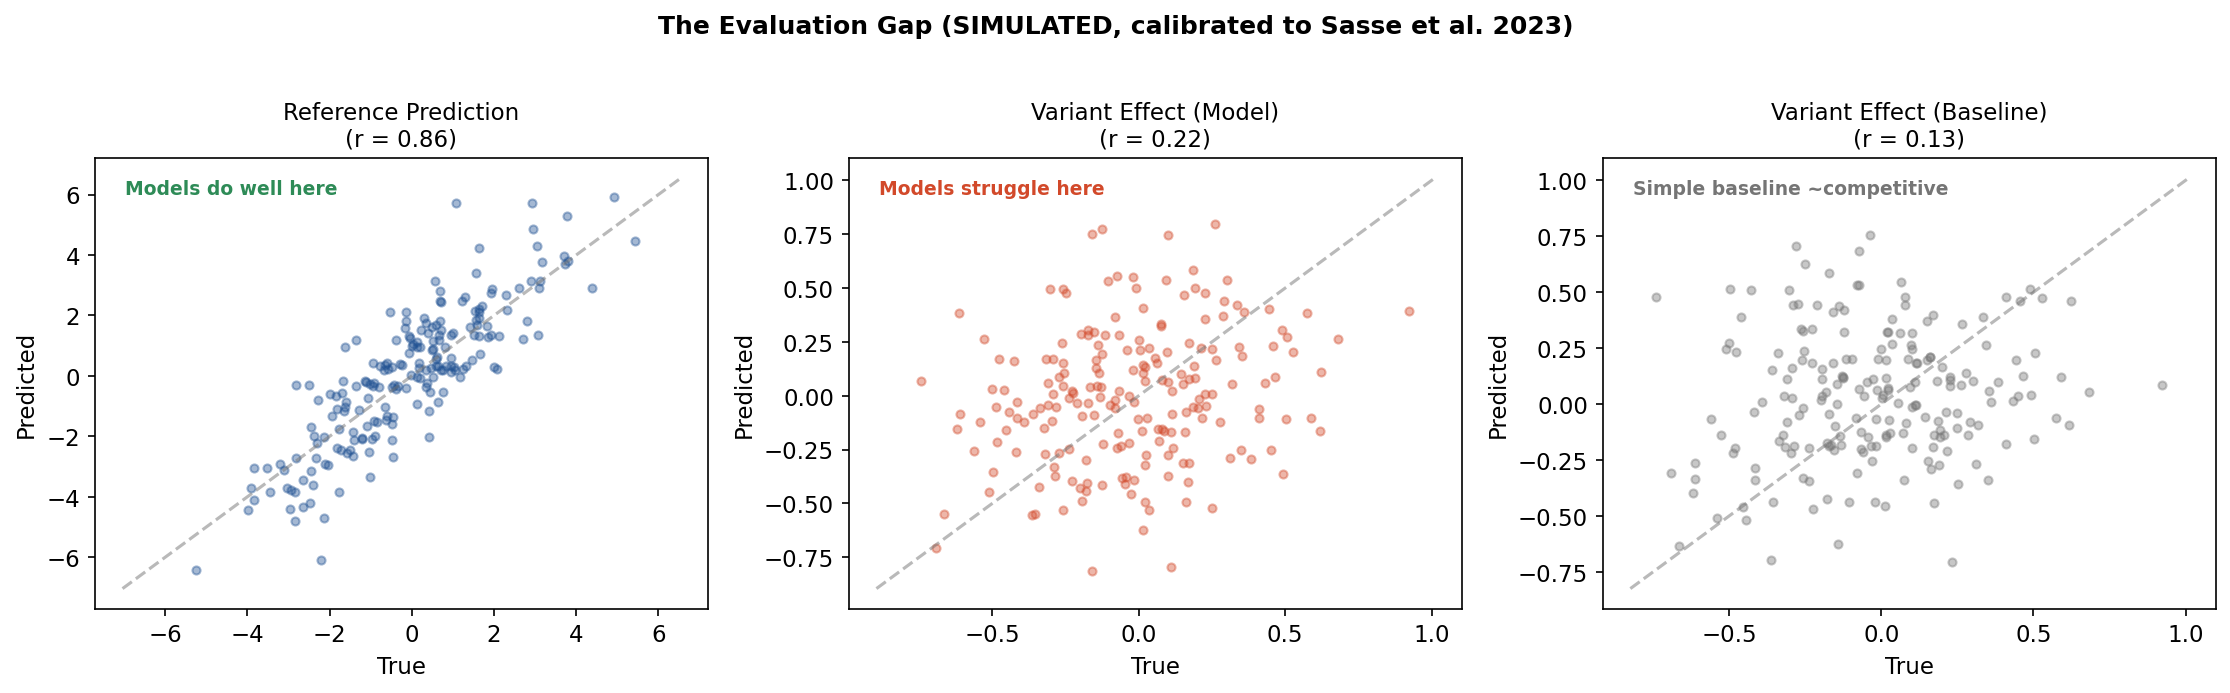
\includegraphics[width=\textwidth,height=0.65\textheight,keepaspectratio]{fig4_dna_fm_evaluation.png}

% \vspace{-0.3em}
% {\scriptsize \textbf{Simulated data} calibrated to Sasse et al.\ (2023). Left: reference expression prediction ($r \sim 0.85$). Center: variant effect prediction ($r \sim 0.15$). Right: simple baseline is competitive. Enformer is too large for Colab; published numbers are printed in the notebook.}
% \end{frame}

\begin{frame}{An Honest Assessment}
\begin{center}
\renewcommand{\arraystretch}{1.15}
{\small
\begin{tabular}{lcc}
\toprule
\textbf{Task} & \textbf{Performance} & \textbf{Clinical Readiness} \\
\midrule
Expression from reference & Strong & Low (not patient-specific) \\
Variant effect (common) & Moderate & Low \\
Variant effect (rare) & Weak & Not ready \\
Regulatory discovery & Promising & Research only \\
\bottomrule
\end{tabular}}
\end{center}
\vspace{0.2em}
Evaluation infrastructure is immature---the field is building benchmarks alongside models.
\vspace{0.2em}

\textbf{Evaluation warning:} If you do not benchmark the clinically relevant target (variant effects), pre-training can look better than it is.
\end{frame}

\section{3D Molecular Models}

\begin{frame}{GNNs on Molecules: Where We Left Off}
\textbf{Recall Lab 12:} You implemented message passing on molecular graphs---atoms as nodes, bonds as edges. GCN and GIN learned to predict blood-brain barrier penetration (BBBP) from 2D molecular topology.

\vspace{0.3em}
\textbf{What Lab 12 covered:}
\begin{itemize}
    \item Graph representation of molecules (adjacency matrix, node features)
    \item Message passing: each node aggregates neighbor information over $K$ rounds
    \item Readout: pool node embeddings $\to$ graph-level prediction
    \item GCN vs.\ GIN architectures; scaffold splits vs.\ random splits
\end{itemize}

\vspace{0.3em}
\textbf{What Lab 12 did not cover:} 3D geometry. Those GNNs operated on 2D topology only---atom types and bond connectivity, no spatial coordinates. Today: what changes when you add the third dimension.
\end{frame}

\begin{frame}{From 2D Graphs to 3D Geometry}
\textbf{The same molecular graph can have different 3D conformations}---a molecule rotated in space has different coordinates but identical properties.

\vspace{0.3em}
\textbf{New features available in 3D:}
\begin{itemize}
    \item Interatomic distances, bond angles, dihedral angles
    \item Spatial proximity (atoms far in the graph may be close in 3D)
\end{itemize}

\vspace{0.2em}
\textbf{New constraint:}
\begin{block}{Invariance vs.\ Equivariance}
Scalar predictions (energy, binding affinity) must be \emph{invariant}: unchanged by rotation. Vector predictions (forces, dipole moments) must be \emph{equivariant}: rotating the input rotates the output in the same way.
\end{block}

{\small Lab 12's fingerprints and 2D GNNs are invariant by construction---they ignore 3D entirely.}
\end{frame}

% \begin{frame}{Why 3D Matters: Chirality}
% \begin{columns}[T]
% \column{0.55\textwidth}
% \begin{center}
% 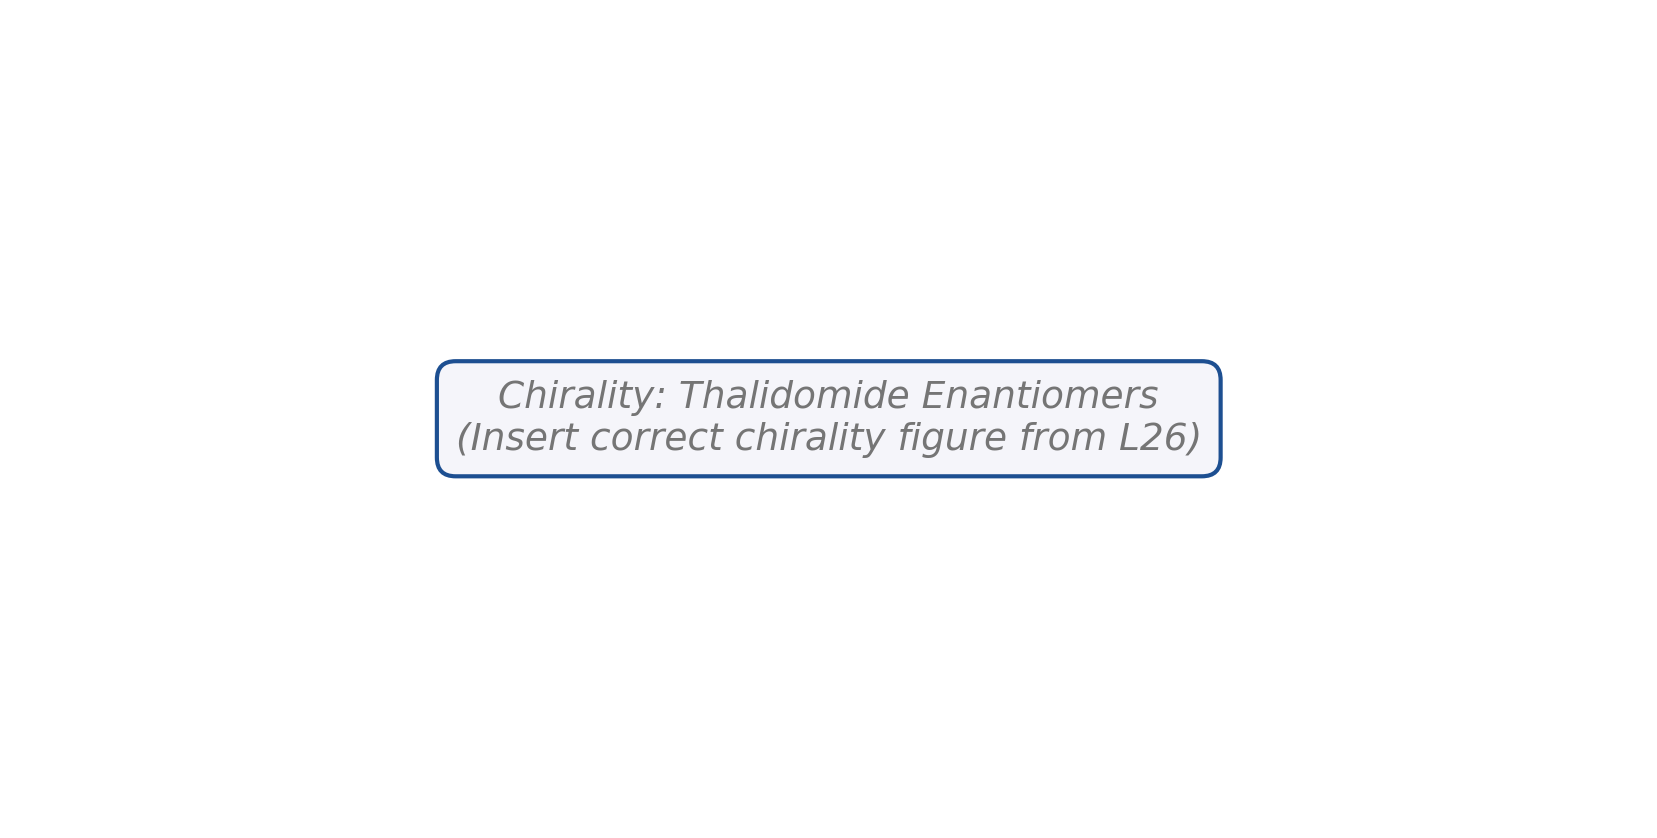
\includegraphics[width=\textwidth,height=0.70\textheight,keepaspectratio]{chirality_placeholder.png}
% \end{center}

% \column{0.42\textwidth}
% \vspace{0.5em}
% \textbf{Same atoms. Same bonds. Same 2D graph. Mirror-image 3D shape.}

% \vspace{0.3em}
% 2D GNNs and Morgan fingerprints cannot distinguish enantiomers---they operate on topology and ignore 3D geometry.

% \vspace{0.3em}
% To predict properties that depend on 3D shape (binding, toxicity, chirality), models must encode spatial geometry explicitly.
% \end{columns}
% \end{frame}

\begin{frame}{Equivariant Neural Networks}
\textbf{Key idea:} Extend Lab 12's message passing to incorporate 3D geometry, while guaranteeing the model respects rotational symmetry.

\vspace{0.2em}
\begin{center}
\renewcommand{\arraystretch}{1.15}
{\small
\begin{tabular}{p{2cm}p{2.5cm}p{2.5cm}p{3.5cm}}
\toprule
\textbf{Model} & \textbf{Inputs} & \textbf{Symmetry handled} & \textbf{Key Idea} \\
\midrule
SchNet & Distances & Rotation, trans. & Continuous-filter conv. \\
DimeNet & Dist. + angles & Same & Directional MP \\
EGNN & Coordinates & SE(3) & Coordinate updates \\
PaiNN & Vectors + scalars & SE(3) & Equivariant MP \\
\bottomrule
\end{tabular}}
\end{center}
\vspace{0.1em}
\textbf{Application:} Classical docking uses physics-based force fields. These models learn the scoring function from data.

\vspace{0.1em}
{\small See Lab 12 for the 2D GNN foundation these build on.}
\end{frame}

\section{Designing New Biology}

\begin{frame}{The Inverse Problem}
\textbf{So far in this lecture:} Predict properties from sequence or structure (the forward problem). \textbf{Biological design:} Generate a sequence or structure that achieves a desired function (the inverse problem).
\begin{center}
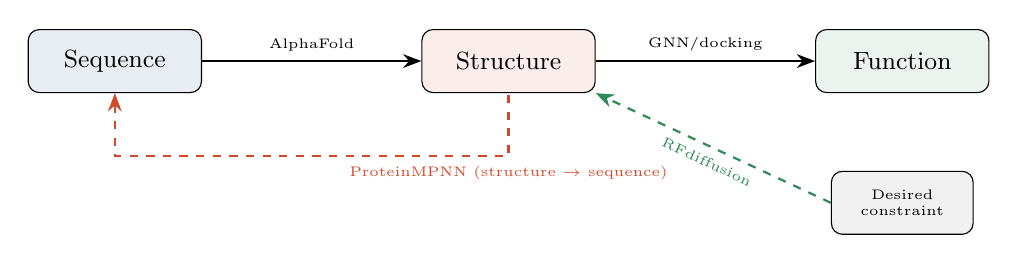
\begin{tikzpicture}[>=Stealth, box/.style={draw,rounded corners,minimum width=2.2cm,minimum height=0.8cm,align=center,font=\small}]
\node[box,fill=columbia!10] (seq) at (0,0) {Sequence};
\node[box,fill=columbiaaccent!10] (str) at (5,0) {Structure};
\node[box,fill=hlgreen!10] (fun) at (10,0) {Function};
\draw[->,thick] (seq) -- (str) node[midway,above,font=\tiny] {AlphaFold};
\draw[->,thick] (str) -- (fun) node[midway,above,font=\tiny] {GNN/docking};
% Inverse arrows
\draw[<-,thick,columbiaaccent,dashed] (seq.south) -- ++(0,-0.8) -| (str.south)
    node[midway,below,font=\tiny] {ProteinMPNN (structure $\to$ sequence)};
% RFdiffusion: constraint-driven generation, not a simple reverse arrow
\node[box,fill=columbiagray!10,font=\tiny,minimum width=1.8cm] (con) at (10,-1.8) {Desired\\constraint};
\draw[->,thick,hlgreen,dashed] (con.west) -- (str.south east)
    node[midway,below,font=\tiny,sloped] {RFdiffusion};
\end{tikzpicture}
\end{center}
{\small Today: designing proteins---same generative principle as molecular generation, but with much stronger structural constraints.}
\end{frame}

\begin{frame}{ProteinMPNN: Inverse Folding}
\textbf{ProteinMPNN} (Dauparas et al., 2022, \textit{Science}) is a DL model for protein sequence design---given a desired 3D backbone, it designs an amino acid sequence that will fold into that shape.

\vspace{0.2em}
\textbf{Input:} 3D backbone coordinates. \textbf{Output:} Sequence that folds there.
\begin{itemize}
    \item Message passing on protein graph (residues = nodes, proximity = edges)
    \item Autoregressive: predict each AA conditioned on structural neighborhood
\end{itemize}
\vspace{0.1em}
{\small Per-residue recovery: $\sim$52\%. Folding success is task/design-set dependent.}
\end{frame}

\begin{frame}{RFdiffusion: Generating New Protein Structures}
\textbf{RFdiffusion} (Watson et al., 2023, \textit{Nature}) generates entirely new protein backbone structures via diffusion---the same generative framework behind image models like DALL-E, applied to 3D protein coordinates.
\begin{center}
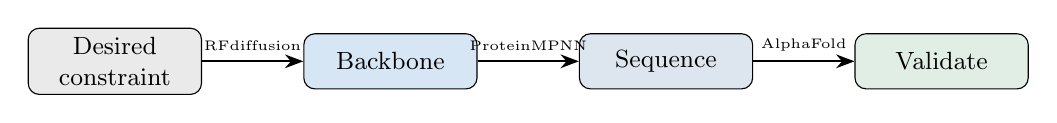
\begin{tikzpicture}[>=Stealth, box/.style={draw,rounded corners,minimum width=2.2cm,minimum height=0.7cm,align=center,font=\small}]
\node[box,fill=columbiagray!15] (con) at (0,0) {Desired\\constraint};
\node[box,fill=columbialight!30] (bb) at (3.5,0) {Backbone};
\node[box,fill=columbia!15] (seq) at (7,0) {Sequence};
\node[box,fill=hlgreen!15] (val) at (10.5,0) {Validate};
\draw[->,thick] (con) -- (bb) node[midway,above,font=\tiny] {RFdiffusion};
\draw[->,thick] (bb) -- (seq) node[midway,above,font=\tiny] {ProteinMPNN};
\draw[->,thick] (seq) -- (val) node[midway,above,font=\tiny] {AlphaFold};
\end{tikzpicture}
\end{center}
\begin{itemize}
    \item Gaussian noise $\to$ iteratively denoise $\to$ protein backbone
    \item Can condition on: target binding site, symmetry, secondary structure
    \item Experimental success: task-dependent ($\sim$10--30\% in early studies)
\end{itemize}
{\small Trained on experimentally determined protein structures. Early evidence these models can generate folds not seen in nature.}
\end{frame}

\begin{frame}{Design Validation}
\textbf{The output of a design model is a hypothesis, not a protein.}
\vspace{0.2em}

\textbf{Computational:} AlphaFold (does it fold right?), ESM (is it plausible?).\\
\textbf{Experimental:} Synthesize $\to$ express $\to$ purify $\to$ test. Weeks to months.
\vspace{0.3em}

Experimental validation rates are highly task-dependent. Computation remains a hypothesis generator; wet-lab filtering is still the bottleneck.
\end{frame}

\begin{frame}{Forward Problems, Inverse Problems, and Causality}
\textbf{A useful analogy:}

\vspace{0.3em}
\begin{center}
\renewcommand{\arraystretch}{1.4}
{\small
\begin{tabular}{p{3.5cm}p{5cm}p{3.5cm}}
\toprule
& \textbf{Biological AI} & \textbf{Clinical ML} \\
\midrule
\textbf{Forward / Predictive} & Sequence $\to$ structure (AlphaFold), sequence $\to$ expression (Enformer) & Patient features $\to$ outcome \\
\textbf{Inverse / Causal} & Desired function $\to$ design a sequence (ProteinMPNN) & Desired outcome $\to$ choose an intervention \\
\bottomrule
\end{tabular}}
\end{center}

\vspace{0.2em}
The forward problem asks: \emph{given this input, what will happen?} Predictive.\\
The inverse problem asks: \emph{what input would produce this outcome?} Structurally similar to causal reasoning---you need a model of how inputs produce outputs, not just correlations.
\end{frame}

\section{Synthesis}

\begin{frame}{What Modern Biological AI Can and Cannot Do}
\begin{itemize}[<+->]
    \item \textbf{Protein LMs (ESM):} Learn coevolution from sequences---effective for well-represented families. Limited for orphan proteins, and sequence plausibility $\neq$ clinical pathogenicity.
    \item \textbf{Structure prediction (AlphaFold):} Highly accurate for globular domains. Not reliable for disorder, dynamics, conformational ensembles.
    \item \textbf{Genomic models (Enformer):} Strong reference expression prediction. Variant effect prediction remains weak---context dependence is invisible.
    \item \textbf{3D molecular models:} Extend 2D GNNs with geometry and symmetry. Powerful for force fields and binding, but classical docking remains competitive.
    \item \textbf{Protein design:} Can generate functional proteins---task-dependent success rates. Demonstrated primarily for simpler topologies so far.
\end{itemize}
\end{frame}

\begin{frame}{The Common Patterns}
Across all biological modalities:
\begin{enumerate}[<+->]
    \item \textbf{Large biological sequence corpora are powerful training data}---via different paradigms (unsupervised LM for ESM, supervised for Enformer, structural supervision for AF2)
    \item \textbf{Evolutionary relatedness provides signal}---explicitly (MSA in AlphaFold), implicitly (sequence distribution in ESM), and sometimes problematically (train/test leakage via phylogenetic relatedness)
    \item \textbf{Geometry becomes increasingly important} from DNA $\to$ proteins $\to$ molecules---equivariance as a design constraint
    \item \textbf{Evaluation lags model development}---benchmarks being built alongside models
    \item \textbf{Classical baselines remain competitive}---MSA-based SIFT, fingerprint QSAR, physics-based docking
\end{enumerate}
\end{frame}

\begin{frame}{Key Takeaways}
Biological ML follows the same arc as clinical ML:
\begin{itemize}[<+->]
    \item \textbf{The evaluation target matters more than the benchmark headline}
    \item \textbf{Pre-training captures useful regularities}, but not necessarily causal mechanisms
    \item \textbf{Architecture encodes domain assumptions:} long context, geometry, equivariance, diffusion---these matter as much as scale
    \item \textbf{Classical baselines remain essential} for calibrating claims
    \item \textbf{Data bias persists:} population bias, assay bias, database bias, and underrepresented biology
\end{itemize}
\end{frame}

\begin{frame}[standout]
    Questions?
\end{frame}

\appendix

\begin{frame}{Appendix: ESM-2 Model Family}
\begin{center}
\renewcommand{\arraystretch}{1.15}
{\small
\begin{tabular}{lrrl}
\toprule
\textbf{Model} & \textbf{Params} & \textbf{Layers} & \textbf{Use Case} \\
\midrule
ESM-2 (8M) & 8M & 6 & Fast demos \\
ESM-2 (35M) & 35M & 12 & \textbf{This notebook} \\
ESM-2 (650M) & 650M & 33 & Strong variant prediction \\
ESM-2 (3B) & 3B & 36 & Best overall, needs GPU \\
\bottomrule
\end{tabular}}
\end{center}
{\small ESM-650M outperforms ESM-3B on some variant effect benchmarks. Bigger is not always better (Lin et al., 2023).}
\end{frame}

\begin{frame}{Appendix: AlphaFold 3}
\textbf{AF3} (Abramson et al., 2024): Protein + ligand + DNA + RNA. Diffusion-based. Public code under restricted non-commercial terms (\texttt{github.com/google-deepmind/alphafold3}).
\end{frame}

% \begin{frame}{Appendix: ESM Embedding t-SNE}
% \centering
% 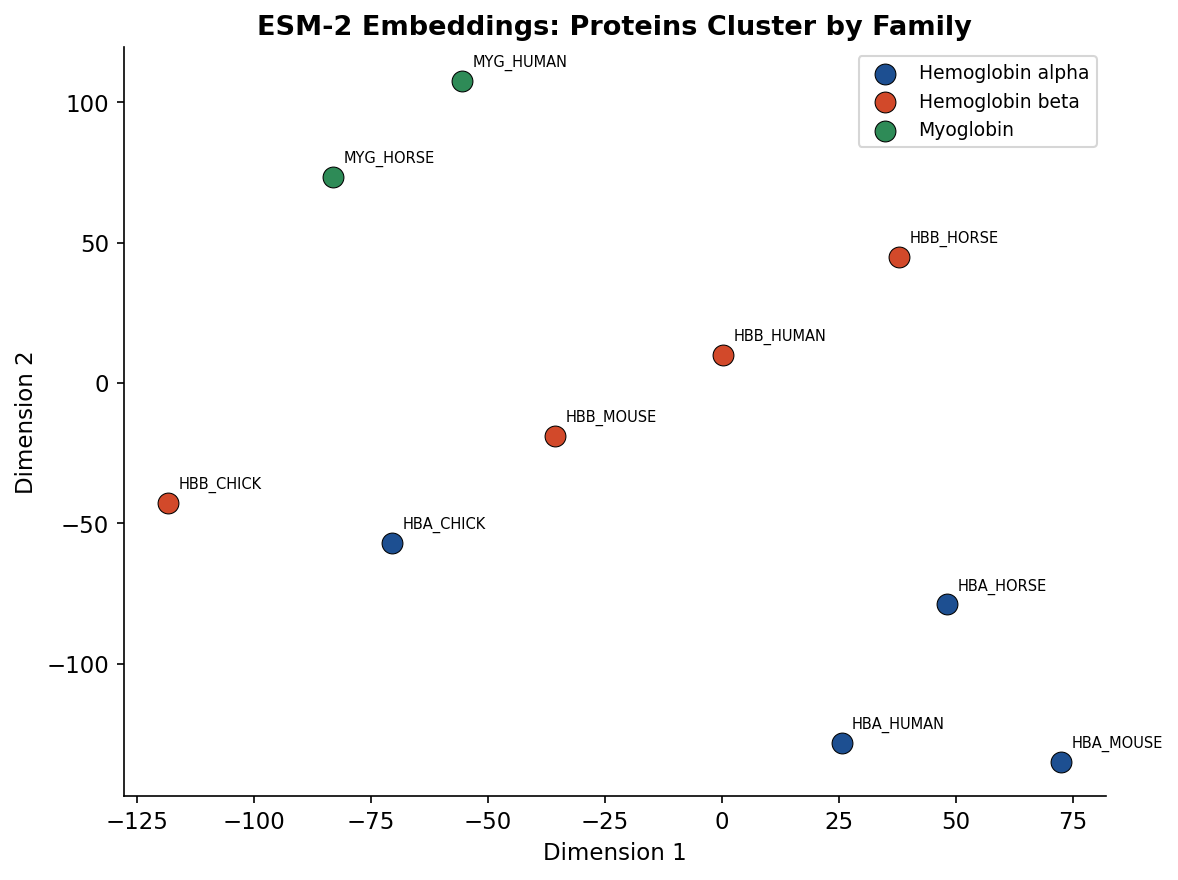
\includegraphics[width=0.55\textwidth,height=0.65\textheight,keepaspectratio]{fig_appendix_tsne.png}

% \vspace{-0.3em}
% {\scriptsize ESM-2 (35M) embeddings for hemoglobin $\alpha$, $\beta$, and myoglobin. Proteins cluster by family---learned from sequence alone.}
% \end{frame}

\end{document}
